\section*{\fontsize{25}{29}\selectfont{\textbf Literature Survey} \\}
{\fontsize{20}{24}\selectfont{\color{red} {RoadRunneR  }}}

\paragraph{} RoadRunneR,lightweight block cipher with the goal of efficiency (especially in 8-bit low cost CPUs) and provable security in terms of minimum number of active S-boxes in differential and linear trails. The cipher is especially designed to have a very low code size, while having high throughput.\\ \\
Our pre- liminary cryptanalysis showed that RoadRunneR have a relatively high security margin in contrast to most lightweight ciphers. RoadRunneR has variable area- time-security trade-off characteristics with different implementation methods so that it can fit the needs of specific application it may be used in.\\ \\
Moreover, we defined a new efficiency comparison metric for block ciphers which (to the best of our knowledge for the first time) takes into account the key size of the cipher. Using this metric, we could compare block ciphers with differ- ent key sizes in a fair way.

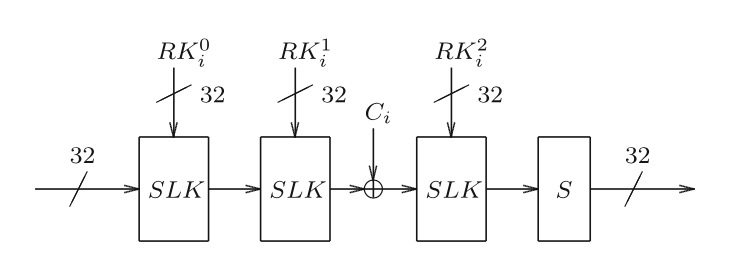
\includegraphics[scale=0.6]{project/images/1.jpg}

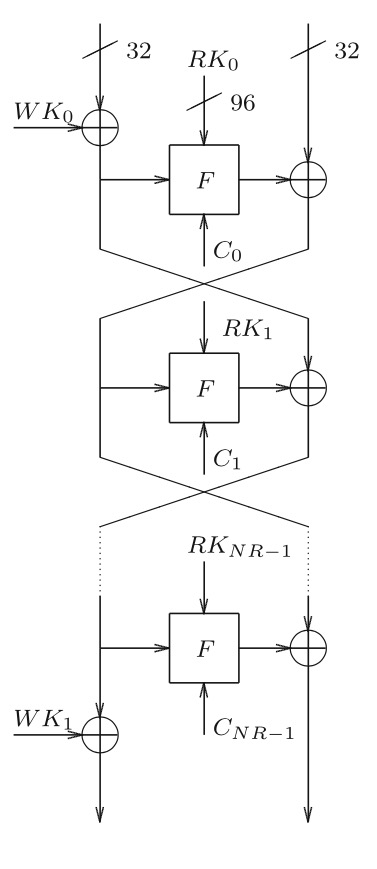
\includegraphics[scale=0.6]{project/images/2.jpg}

This is the  internal structure of the function F in figure 1 that is basically a SLK function that is the consecutive application of S-box layer(S) ,Diffusion Layer(L) and Key addition (K).


\section*{\fontsize{20}{24}\selectfont{\color{red} {Substitution and Diffusion:}}}

When X (figure 1) that is basically a 32 bit when going into F function then first it will go to the S -box which is basically the following:

{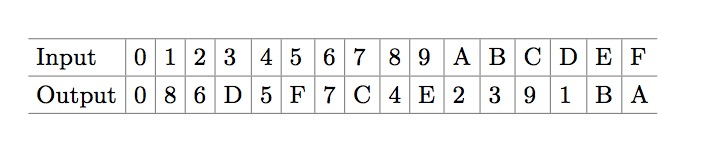
\includegraphics[scale=0.6]{project/images/4.jpg}}

Bit slice S-box structure has advantage in both hardware and software implementations. In software, the per- mutations before and after the S-boxes disappear. In hardware, on the other hand, they can be implemented by a simple wiring which consumes no extra area. 

The bits(permutation) gets substituted according to the S-box and a new permutation is formed after coming out from the S-box which is followed by the diffusion in the L box as follows:

After the bitslice S-box layer, we used a linear function on each byte of the state to provide diffusion inside 8-bit words. 

So we needed an efficient linear function operating on bytes. One classical solution for such a linear function for CPUs is using XOR of shifted and rotated values of the input word. 

We try to build linear functions of the form :

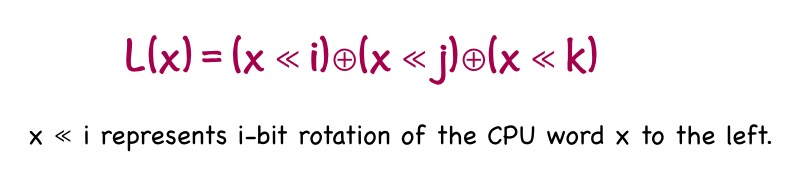
\includegraphics[scale=0.5]{project/images/5.jpg}

\section*{\fontsize{20}{24}\selectfont{\color{red} {Key Addition:}}}\\

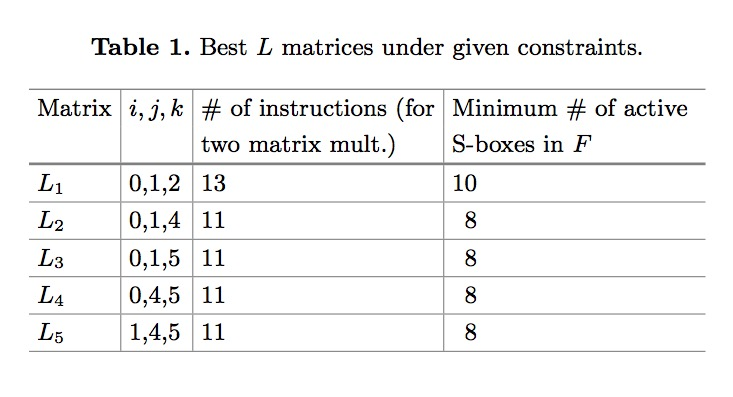
\includegraphics[scale=0.6]{project/images/6.jpg}

For example, if master key is 128-bit, it will be divided into 4 words of 32-bit as A∥B∥C∥D. Initial whitening key is A, first round key is B-C-D, second round key is A-B-C, etc. 

We call it as Whitening Key because its basic  function is to xor the initial bits in round 1 and the final bits after the last round.

\section*{\fontsize{20}{24}\selectfont{\color{red} {What Ci Represents?}}}\\

After the second SLK function, round constant is XORed to the least significant byte (rightmost byte, i.e., x3) of the state. For round i = 0,1,...,NR − 1, the round constant is Ci = NR − i, where NR is the number of rounds, and Ci is represented as 8-bit little endian integer, that is 12 = 00001100, 11 = 00001011, etc. 


